%% !TEX program = xelatex
%% !BIB program = bibtex
\documentclass[10pt,aspectratio=169]{beamer}  % present

\mode<presentation>
{
    \usetheme{default}   % or try Boadilla, boxes, Singapore, Darmstadt, Madrid, Warsaw, ...
    \usecolortheme{default} % or try albatross, beaver, crane, ...

    \usefonttheme{structurebold}  % or try serif, , ...
    \setbeamertemplate{navigation symbols}{}
    \setbeamertemplate{caption}[numbered]
    \definecolor{MyColor}{rgb}{0,0.3,0.65}
    \definecolor{MyColorLight}{rgb}{0,0.7,0.95}
    \definecolor{MyGreenColor}{rgb}{0,0.6,0}
    \definecolor{MyRedColor}{rgb}{0.8,0,0}
    \setbeamercolor{structure}{fg=MyColor}
}

%% Packages
\usepackage[round]{natbib}
%\usepackage{authblk}
\usepackage{amsfonts,amsmath,amssymb,mathtools,marvosym,amsthm,ulem,cancel}
%\usepackage{enumerate}
\usepackage{graphicx,float,tcolorbox}
\hypersetup{colorlinks,linkcolor=MyColor,citecolor=MyColor,urlcolor=black,breaklinks=true}
% \usepackage{fontspec}
% \usepackage{tikz}

%% Print author name, short title, date and slide number at the bottom of the page
% \setbeamercolor{author in head/foot}{fg=MyColor, bg=MyColorLight}
\makeatletter
\setbeamertemplate{footline}
{
    \leavevmode%
    \hbox{%
        \begin{beamercolorbox}[wd=.333333\paperwidth,ht=2.25ex,dp=1ex,center]{author in head/foot}%
            \usebeamerfont{author in head/foot}\insertshortauthor
        \end{beamercolorbox}%
        \begin{beamercolorbox}[wd=.333333\paperwidth,ht=2.25ex,dp=1ex,center]{title in head/foot}%
            \usebeamerfont{title in head/foot}\insertshorttitle
        \end{beamercolorbox}%
        \begin{beamercolorbox}[wd=.333333\paperwidth,ht=2.25ex,dp=1ex,right]{date in head/foot}%
            \usebeamerfont{date in head/foot}\insertshortdate{}\hspace*{2em}
            \insertframenumber{} / \inserttotalframenumber\hspace*{2ex}
        \end{beamercolorbox}%
    }%
    \vskip0pt%
}
\makeatother

% \setmainfont{Ubuntu}
% \setmainfont{DejaVu Serif}
% \setsansfont{Segoe UI}
% \setsansfont{EB Garamond}
% \setsansfont{Tahoma}
% \setsansfont{Roboto}
% \setsansfont{Open Sans}
% \setsansfont{Georgia}
% \setsansfont{SF Pro Display}
% \setsansfont{Lato}
% \setmonofont{Monospaced}


%\setlength{\parindent}{0.5cm}
\setlength{\parskip}{0.3cm}

\renewcommand{\baselinestretch}{1.0}
\renewcommand{\arraystretch}{1.2}

\newtheorem{proposition}{Proposition}

% ------------------------------------------------------------------------------

%% Description
\author[Narek Ohanyan]{Narek Ohanyan}
\title[Lecture 4. Unit Root Tests for Stationarity]{Lecture 4. Unit Root Tests for Stationarity}
\institute[AUA]{American University of Armenia}
\date{\today}

% ------------------------------------------------------------------------------

%% Add table of contents before every subsection
\AtBeginSection[]
{
    \begin{frame}{Outline}
        \tableofcontents[currentsection]
    \end{frame}
}

% ==============================================================================

\begin{document}

\begin{frame}
    \titlepage
\end{frame}

% ==============================================================================

\section{Non-stationary Processes}

% ------------------------------------------------------------------------------

\begin{frame}{Trend-stationary processes}

    \bigskip
    The time series $ y_{t} $ is called \textbf{trend stationary} if it is stationary around a deterministic trend.

    \medskip
    Consider the following time series model
    \begin{align*}
        \qquad\qquad\qquad\qquad y_{t}                          & = \alpha + \beta t + x_{t}                                                      \\
        x_{t} & = \phi x_{t-1} + e_{t} \qquad e_{t} \sim \text{WN} \left( 0, \sigma^{2} \right)
    \end{align*}

    In other words, $ y_{t} $ is trend stationary if after removing the trend $ \alpha + \beta t $, the resulting series $ x_{t} $ is stationary.

    \medskip
    We can also write the model as
    \begin{align*}
        y_{t} & = \gamma_0 + \phi y_{t-1} + \gamma_1 t + e_{t}
    \end{align*}
    where $ \gamma_0 = \alpha \left( 1 - \phi \right) + \phi \beta $ and $ \gamma_1 = \beta \left( 1 - \phi \right) $.

\end{frame}

% ------------------------------------------------------------------------------

\begin{frame}{An example of a trend-stationary process}

    \bigskip
    \begin{figure}[H]
        \centering
        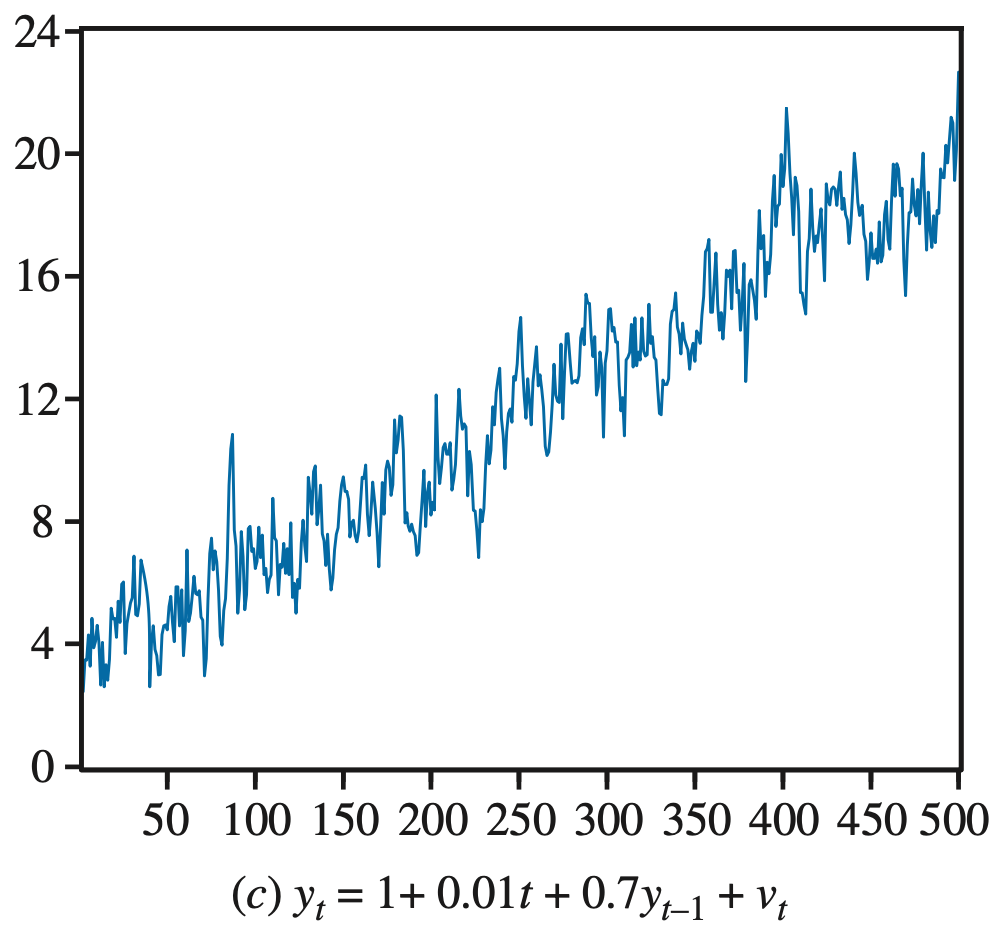
\includegraphics[height=0.5\textwidth]{./fig/trend-stationary.png}
    \end{figure}

\end{frame}

% ------------------------------------------------------------------------------

\begin{frame}{Random-walk processes}

    \bigskip
    The time series $ y_{t} $ is called a \textbf{random walk} if it has the following form
    \begin{align*}
        \qquad\qquad\qquad\qquad y_{t} = y_{t-1} + e_{t} \qquad e_{t} \sim \text{WN} \left( 0, \sigma^{2} \right)
    \end{align*}

    The random walk process may be written as
    \begin{align*}
        y_{t} & = y_{0} + \sum_{i=1}^{t} e_{i}
    \end{align*}
    The term $ \sum_{i=1}^{t} e_{i} $ is called the \textbf{stochastic trend}.

    \medskip
    Random walk process has the following properties
    \begin{align*}
        \mathrm{E} \left( y_{t} \right) = y_{0} \qquad\qquad \mathrm{Var} \left( y_{t} \right) = t \sigma^{2} \qquad\qquad \mathrm{Cov} \left( y_{t}, y_{t-k} \right) = \left( t-k \right) \sigma^{2}
    \end{align*}

\end{frame}

% ------------------------------------------------------------------------------

\begin{frame}{An example of a random walk process}

    \bigskip
    \begin{figure}[H]
        \centering
        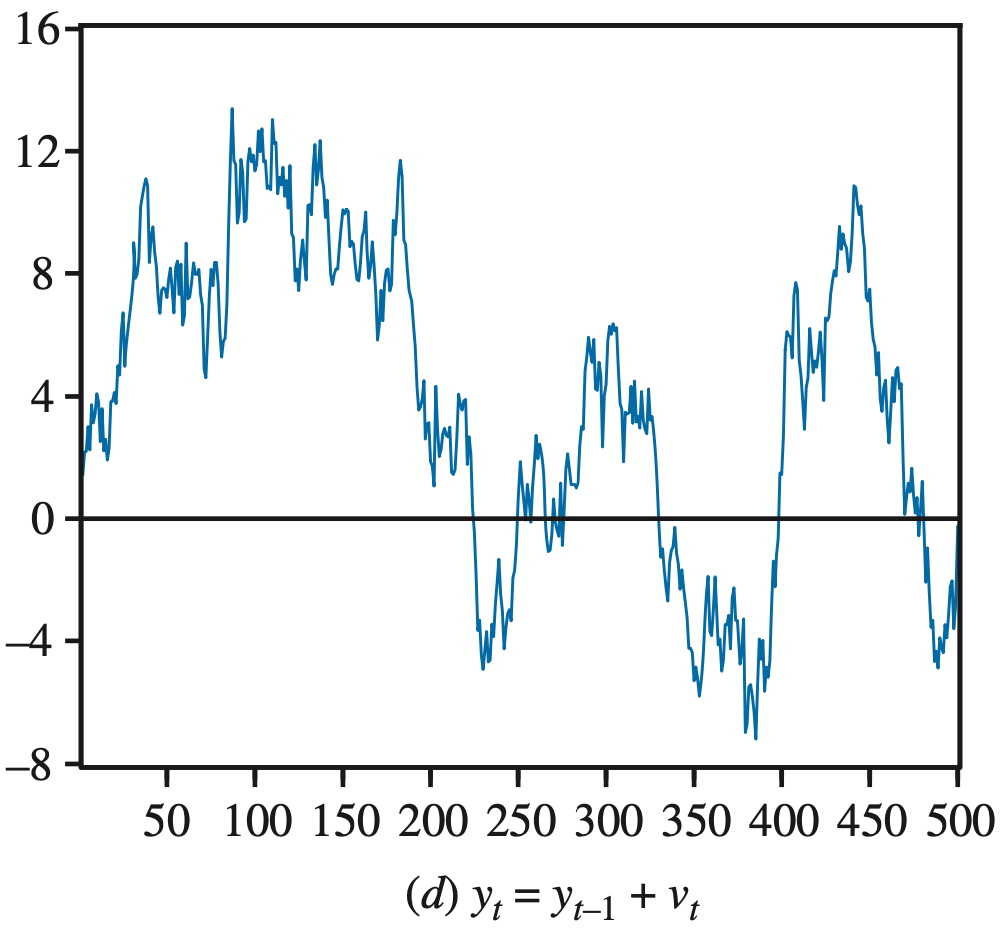
\includegraphics[height=0.5\textwidth]{./fig/random-walk.png}
    \end{figure}

\end{frame}

% ------------------------------------------------------------------------------

\begin{frame}{Random-walk with drift}

    \bigskip
    The time series $ y_{t} $ is called a \textbf{random walk with drift} if it has the following form
    \begin{align*}
        \qquad\qquad\qquad\qquad y_{t} = \alpha + y_{t-1} + e_{t} \qquad e_{t} \sim \text{WN} \left( 0, \sigma^{2} \right)
    \end{align*}

    The random walk process may be written as
    \begin{align*}
        y_{t} & = y_{0} + \alpha t + \sum_{i=1}^{t} e_{i}
    \end{align*}
    The term $ \alpha t $ is called the \textbf{deterministic trend}.

    \medskip
    Random walk process has the following properties
    \begin{align*}
        \mathrm{E} \left( y_{t} \right) = y_{0} + \alpha t \qquad\qquad \mathrm{Var} \left( y_{t} \right) = t \sigma^{2} \qquad\qquad \mathrm{Cov} \left( y_{t}, y_{t-k} \right) = \left( t-k \right) \sigma^{2}
    \end{align*}

\end{frame}

% ------------------------------------------------------------------------------

\begin{frame}{An example of a random walk with drift process}

    \bigskip
    \begin{figure}[H]
        \centering
        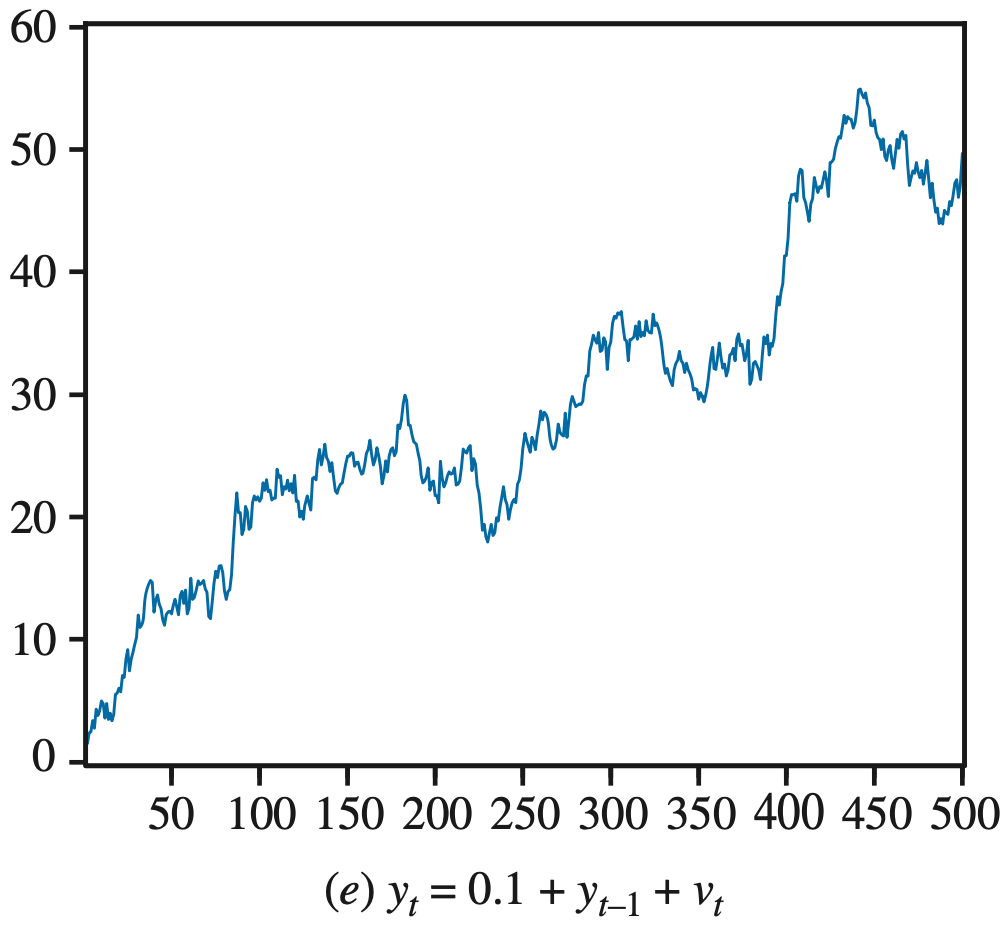
\includegraphics[height=0.5\textwidth]{./fig/random-walk-drift.png}
    \end{figure}

\end{frame}

% ==============================================================================

\section{Spurious Regressions}

% ------------------------------------------------------------------------------

\begin{frame}{Spurious regressions}

    \bigskip
    Regressions of non-stationary time series may produce \textbf{spurious} results.

    \medskip
    Consider two independent random walks
    \begin{align*}
        \qquad\qquad\qquad\qquad y_{t} & = y_{t-1} + e_{t} \qquad e_{t} \sim \text{WN} \left( 0, \sigma^{2} \right) \\
        x_{t}                          & = x_{t-1} + u_{t} \qquad u_{t} \sim \text{WN} \left( 0, \sigma^{2} \right)
    \end{align*}

    The regression of $ y_{t} $ on $ x_{t} $ will likely produce a high $ R^{2} $ and significant $ t $-statistics.

    \medskip
    The problem is that both $ y_{t} $ and $ x_{t} $ are non-stationary, and the regression is spurious.

\end{frame}

% ------------------------------------------------------------------------------

\begin{frame}{Example of two independent random walks}

    \bigskip
    \begin{figure}[H]
        \centering
        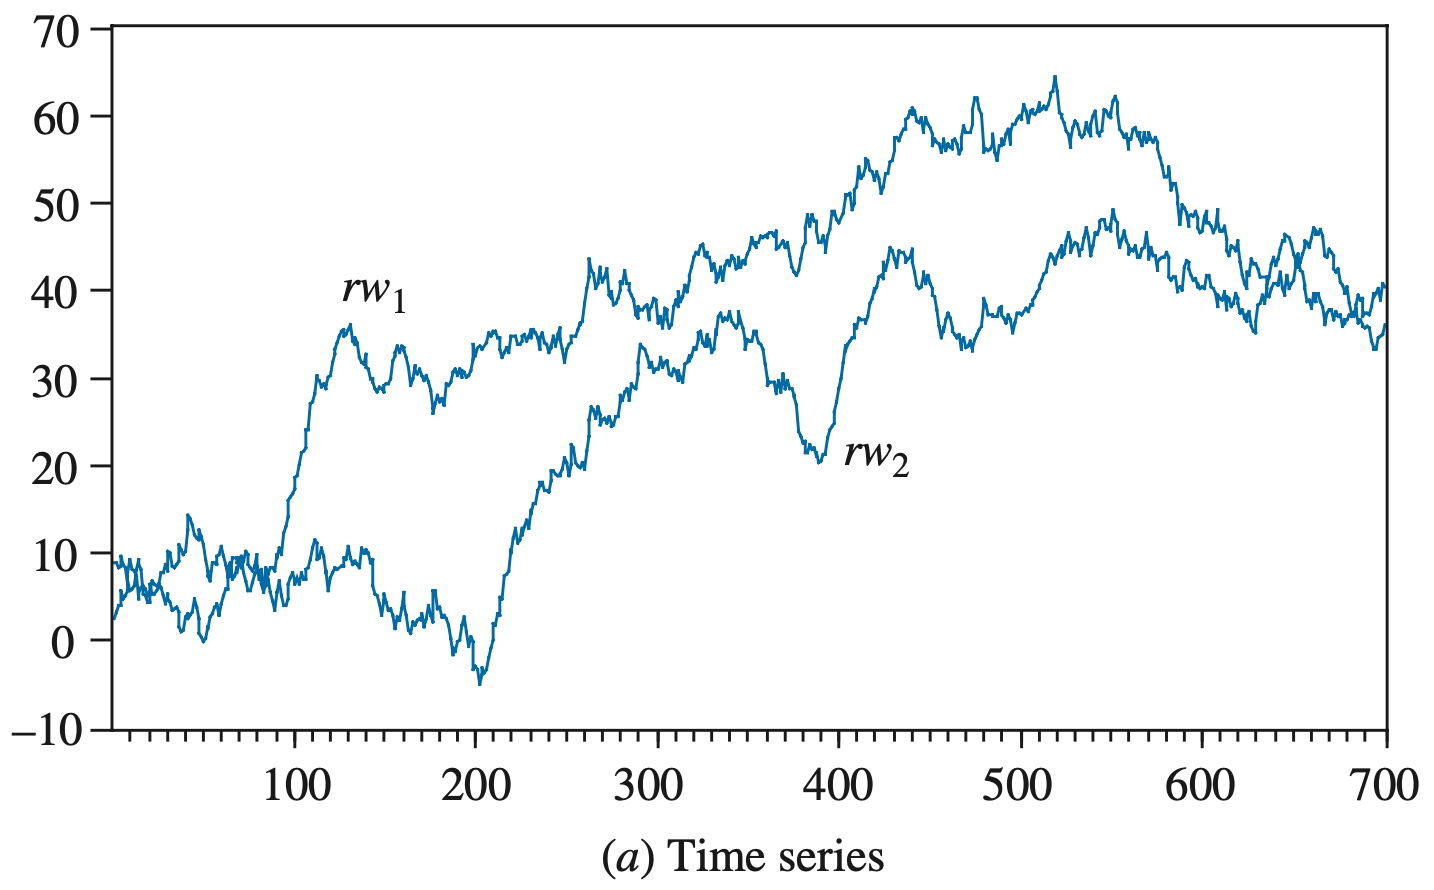
\includegraphics[height=0.5\textwidth]{./fig/rwq-rw2-series.png}
    \end{figure}

\end{frame}

% ------------------------------------------------------------------------------

\begin{frame}{Scatter plot of two independent random walks}

    \bigskip
    \begin{figure}[H]
        \centering
        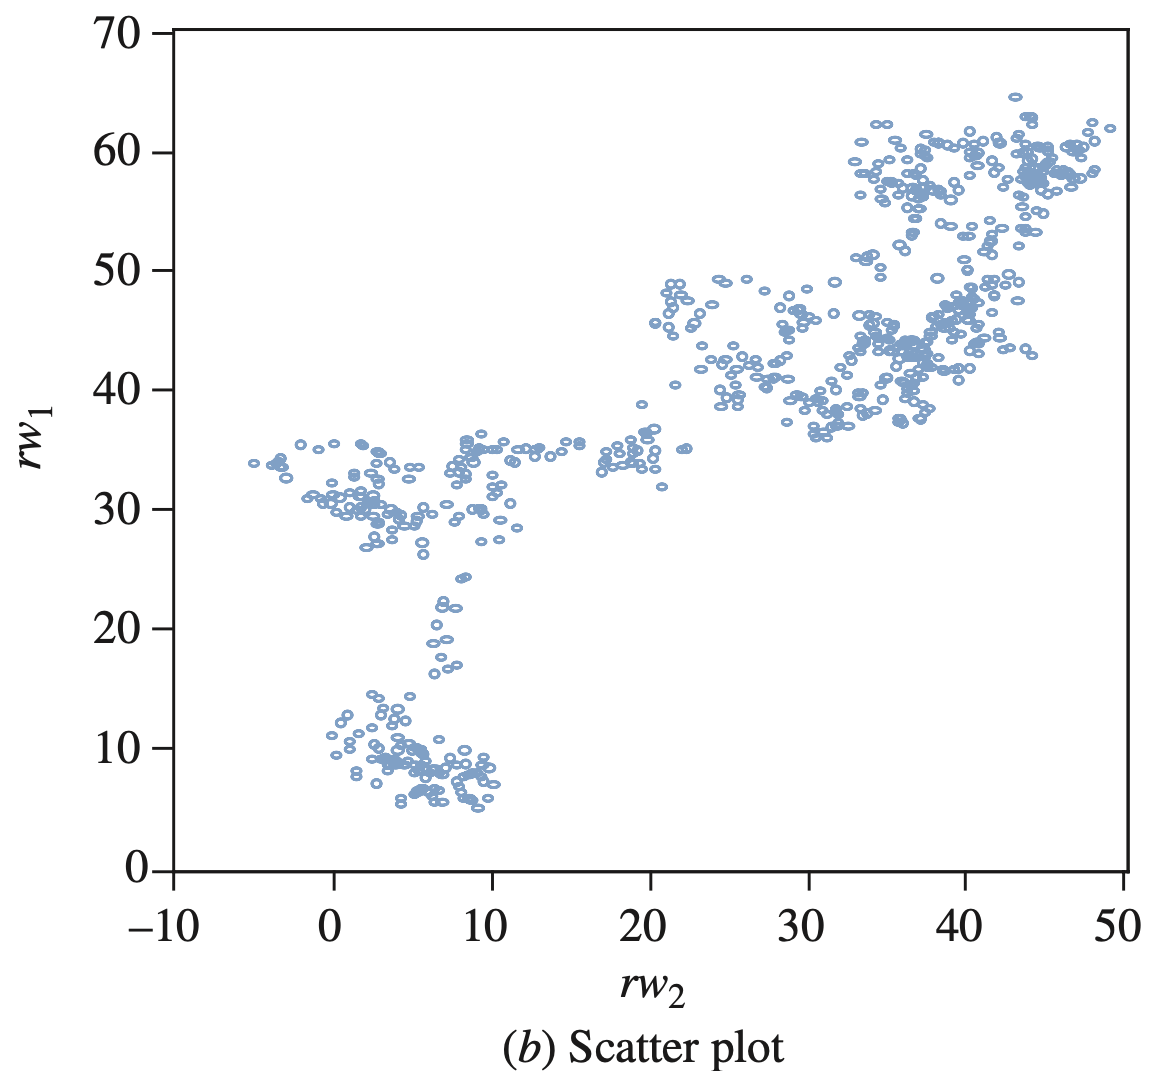
\includegraphics[height=0.5\textwidth]{./fig/rwq-rw2-scatter.png}
    \end{figure}

\end{frame}

% ==============================================================================

\section{Unit Root Tests}

% ------------------------------------------------------------------------------

\begin{frame}{Unit root tests}

    \bigskip
    Recall that an AR(1) process is given by
    \begin{align*}
        y_{t} & = \phi y_{t-1} + e_{t} \qquad e_{t} \sim \text{WN} \left( 0, \sigma^{2} \right)
    \end{align*}

    When $ \phi = 1 $, the process is called a \textbf{unit root} process.

    \medskip
    The most popular test for unit root is the \textbf{Dickey-Fuller test} for the hypothesis
    \begin{align*}
        \mathrm{H}_0: \phi = 1 \qquad \text{vs.} \qquad \mathrm{H}_1: \phi < 1
    \end{align*}

    Other tests include the \textbf{Phillips-Perron test}, the \textbf{Kwiatkowski-Phillips-Schmidt-Shin test}, and the \textbf{Elliott-Rothenberg-Stock test}.

\end{frame}

% ------------------------------------------------------------------------------

\begin{frame}{Dickey-Fuller test}

    \bigskip
    The Dickey-Fuller test is based on the following alternative models
    \begin{itemize}
        \item No constant, no trend
              \begin{align*}
                  \Delta y_{t} & = \gamma y_{t-1} + e_{t}
              \end{align*}
        \item Constant, no trend
              \begin{align*}
                  \Delta y_{t} & = \alpha + \gamma y_{t-1} + e_{t}
              \end{align*}
        \item Constant and trend
              \begin{align*}
                  \Delta y_{t} & = \alpha + \gamma y_{t-1} + \lambda t + e_{t}
              \end{align*}
    \end{itemize}

    The hypothesis of the tests is
    \begin{align*}
        \mathrm{H}_0: \gamma = 0 \qquad \Longleftrightarrow \qquad \mathrm{H}_0: \phi = 1 \\
        \mathrm{H}_1: \gamma < 0 \qquad \Longleftrightarrow \qquad \mathrm{H}_1: \phi < 1
    \end{align*}

\end{frame}

% ------------------------------------------------------------------------------

\begin{frame}{AR processes and the Dickey-Fuller tests}

    \bigskip
    \begin{figure}[H]
        \centering
        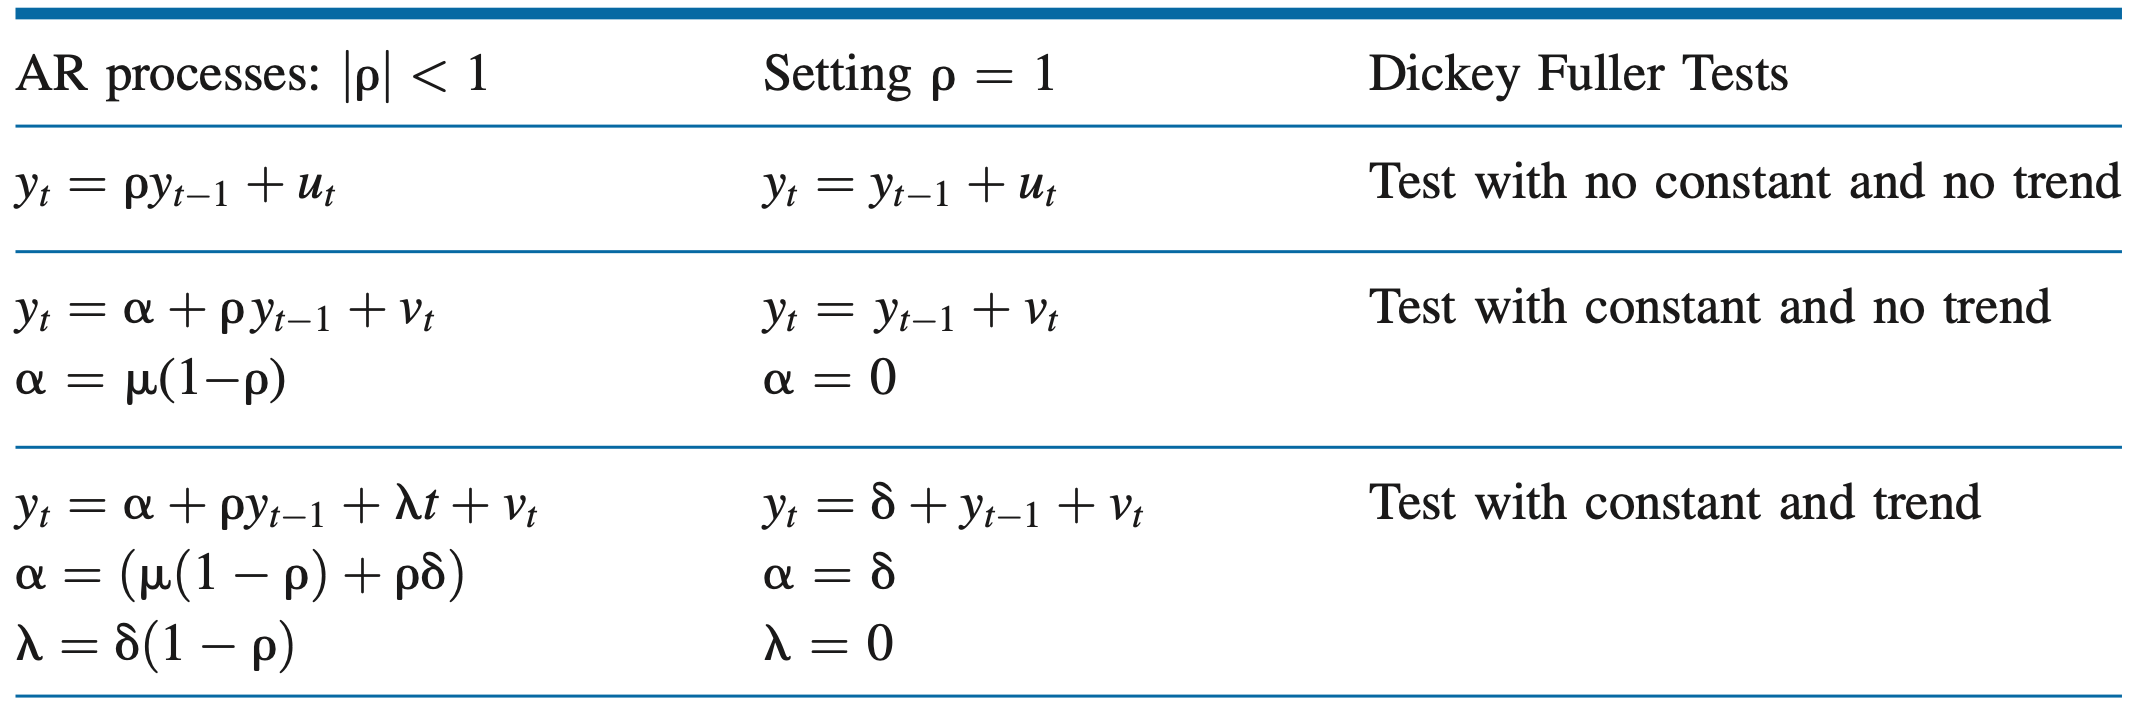
\includegraphics[height=0.3\textwidth]{./fig/dickey-fuller-hypotheses.png}
    \end{figure}

\end{frame}

% ------------------------------------------------------------------------------

\begin{frame}{Distribution of the test statistic}

    \bigskip
    The Dickey-Fuller test equation is estimated by OLS, and the test statistic is
    \begin{align*}
        \tau & = \frac{\hat{\gamma}}{\mathrm{se} (\hat{\gamma})}
    \end{align*}
    where $ \hat{\gamma} $ is the OLS estimate of $ \gamma $, and $ \mathrm{se} (\hat{\gamma}) $ is the standard error of the estimate.

    \medskip
    Under the null hypothesis, the test statistic has a non-standard distribution.

    \medskip
    The null hypothesis is rejected if $ \tau < \tau_{c} $, where $ \tau_{c} $ depends on the type of the model used.

\end{frame}

% ------------------------------------------------------------------------------

\begin{frame}{Critical values of the Dickey-Fuller test}

    \bigskip
    \begin{figure}[H]
        \centering
        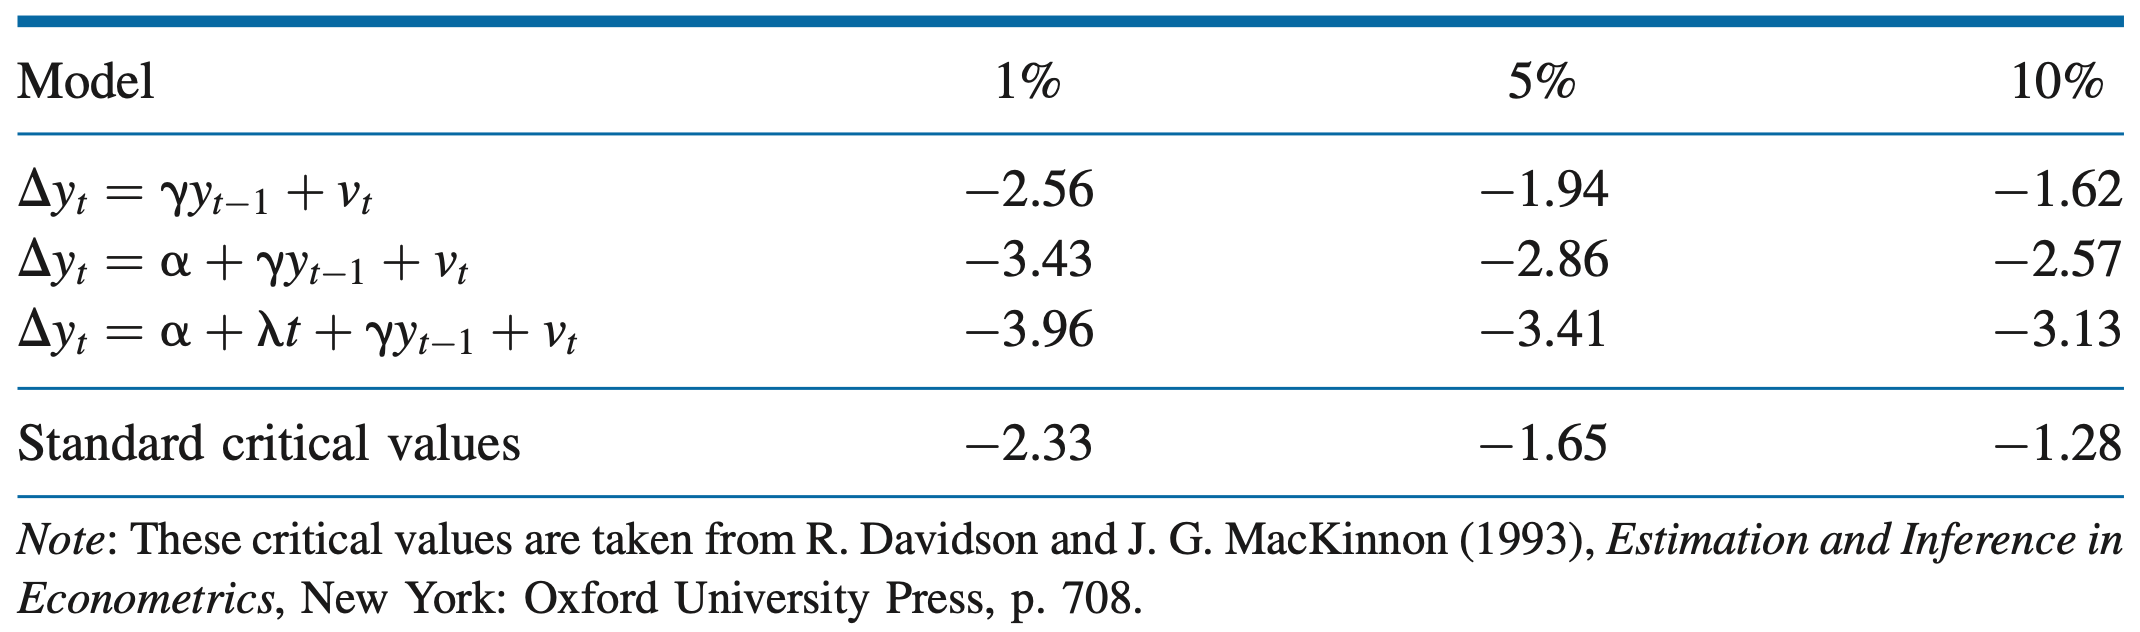
\includegraphics[height=0.25\textwidth]{./fig/dickey-fuller-critical-values.png}
    \end{figure}

\end{frame}

% ------------------------------------------------------------------------------

\begin{frame}{Augmented Dickey-Fuller test}

    \bigskip
    The \textbf{Augmented Dickey-Fuller (ADF)} test is a generalization of the Dickey-Fuller test.

    \medskip
    The ADF test includes additional lags of the dependent variable in the regression equation
    \begin{align*}
        \Delta y_{t} & = \alpha + \gamma y_{t-1} + \sum_{i=1}^{p} \delta_{i} \Delta y_{t-i} + e_{t}
    \end{align*}

    Inclusion of additional lags aims to eliminate the \textit{serial correlation} in the error term.

    \medskip
    The number of lags $ p $ is chosen based on the AIC or BIC criteria.

\end{frame}

% ==============================================================================

\section{Integrated Processes}

% ------------------------------------------------------------------------------

\begin{frame}{Integrated processes}

    \bigskip
    Recall that if $ y_{t} $ follows a random walk, then $ \Delta y_{t} $ is \begin{align*}
        \Delta y_{t} = y_{t} - y_{t-1} = e_{t}
    \end{align*}
    which is stationary.

    A time series $ y_{t} $ is called \textbf{integrated} of order one, denoted as $ I(1) $, if its first difference is stationary.

    \medskip
    In general, a time series $ y_{t} $ is called \textit{integrated} of order $ d $, denoted as $ I(d) $, if its $ d $-th difference is stationary
    \begin{align*}
        \Delta^{d} y_{t} = \Delta \left( \Delta^{d-1} y_{t} \right)
    \end{align*}

    The order of integration $ d $ is the number of times the series must be differenced to obtain a stationary series.

\end{frame}

% ------------------------------------------------------------------------------

\begin{frame}{ARIMA models}

    \bigskip
    The \textbf{Autoregressive Integrated Moving Average (ARIMA)} model is a generalization of the ARMA model.

    \medskip
    The $ \text{ARIMA} (p, d, q) $ model is given by
    \begin{align*}
        \qquad\qquad x_{t} & = \phi_1 x_{t-1} + \ldots + \phi_p x_{t-p} + e_{t} + \theta_1 e_{t-1} + \ldots + \theta_q e_{t-q} \qquad e_{t} \sim \text{WN} \left( 0, \sigma^{2} \right)
    \end{align*}
    where $ x_{t} = \Delta^{d} y_{t} $.

    \medskip
    ARIMA models are estimated by \textbf{Maximum Likelihood Estimation (MLE)}.

    \medskip
    Prior to estimation, $ d $ must be determined by the ADF test, and the $ p $ and $ q $ are chosen based on the AIC or BIC criteria.

\end{frame}

% ==============================================================================

% % \begin{frame}<beamer:0>
% \begin{frame}[allowframebreaks]{Bibliography}

%     \bibliographystyle{apalike}
%     \bibliography{references}

% \end{frame}

% ==============================================================================

\end{document}
